% This is samplepaper.tex, a sample chapter demonstrating the
% LLNCS macro package for Springer Computer Science proceedings;
% Version 2.20 of 2017/10/04
%
\documentclass[runningheads]{llncs}
%------------------------------------------------------------------------------------- (LIBRARIIES)
\usepackage{graphicx}
\usepackage{listings}
\usepackage{color}
\usepackage{hyperref}
% to display URLs in blue roman font according to Springer's eBook style:
\renewcommand\UrlFont{\color{blue}\rmfamily}
\usepackage{subfigure}
\usepackage{listings}
\usepackage[english]{babel}

% Default fixed font does not support bold face
\DeclareFixedFont{\ttb}{T1}{txtt}{bx}{n}{12} % for bold
\DeclareFixedFont{\ttm}{T1}{txtt}{m}{n}{12}  % for normal

% Custom colors
\definecolor{deepblue}{rgb}{0,0,0.5}
\definecolor{deepred}{rgb}{0.6,0,0}
\definecolor{lessdeepred}{rgb}{0.3,0,0}
\definecolor{deepgreen}{rgb}{0,0.5,0}


%------------------------------------------------------------------------------------- (Python)
% Python style for highlighting
\newcommand\pythonstyle{\lstset{
language        =Python,
basicstyle      =\fontsize{7}\ttm,
morekeywords    ={self},              % Add keywords here
keywordstyle    =\fontsize{7}\ttb\color{deepblue},
emph            ={MyClass,FeatureExtractor,__init__, None, True},        % Custom highlighting
emphstyle       =\fontsize{7}\ttb\color{deepred},    % Custom highlighting style
stringstyle=\color{deepgreen},
frame=tb,                         % Any extra options here
showstringspaces=false
}}

% Python environment
\lstnewenvironment{python}[1][]
{
\pythonstyle
\lstset{#1}
}
{}

% Python for external files
\newcommand\pythonexternal[2][]{{
\pythonstyle
\lstinputlisting[#1]{#2}}}

% Python for inline
\newcommand\pythoninline[1]{{\pythonstyle\lstinline!#1!}}


%------------------------------------------------------------------------------------- (Dokument)
\begin{document}

\title{Digital Libraries - Document Fingerprints}

%------------------------------------------------------------------------------------- (Title)
\author{Richard Hohensinner\inst{1}\orcidID{00273237} \and \\
Inti Gabriel Mendoza Estrada\inst{1}\orcidID{11804156} \and     \\
Jürgen Suntinger-Schrampf\inst{1}\orcidID{00630894}}

\authorrunning{R. Hohensinner et al.}
% First names are abbreviated in the running head.
% If there are more than two authors, 'et al.' is used.
\institute{TU Graz, Austria \\ GROUP 11}
\maketitle              % typeset the header of the contribution


%------------------------------------------------------------------------------------- (Abstract)
\begin{abstract}
The human is the best pattern recognition system in the whole world and has no problems when it comes to detecting outliers or finding patterns in a visual way. However, when it comes to textual data, the human brain has problems detecting or recognizing such things in an efficient way. At this point, the computer comes into play which extracts a sum of so called features (characteristics), which can then be illustrated just the way the human prefers it most, Visually. In our case, that happened through heatmaps which should help the user to do a visual analysis under the help of interactive tools to find the so called literal-\textbf{fingerprints} (characteristic) of an author.

\end{abstract}
\keywords{Document fingerprint  \and Digital libraries \and Visualisation}


%------------------------------------------------------------------------------------- (Introduction)
\section{Introduction}
As the world enters an era defined by \textit{big data}, more and more information is being actively accrued. This vast amount of data is not immediately available to people. It must now be accessible. What libraries did for physical books, digital libraries are doing for digital data. Challenges begin to appear when you consider that data can come in a vast array of ways (on top of the actual amount of data). When challenges appear, however, their solutions end up, most often than not, incredibly useful. Digital libraries not only let you access texts, papers, books. You are able to access videos, images, 3D models\ldots What makes digital libraries so incredibly useful lies in the fields it comprises: Computer Science, Information Science, and Information Visualisation - to name a few. 

In Computer Science comes something called \textit{Natural Language Processing} (or NLP). NLP is the automatic understanding of text by a computer. Being able to "understand" text is immensely useful. In the field of Digital Libraries, therefore, you can not only access text via keywords or titles but also through what the text actually means and compels.

What if you could search through a text based on the emotions of sentences? What if you could find texts that are easy to read based on sentence length? What if you could find texts to improve your language skills based on sentence complexity? What if you could use NLP to train a Neural Network to guess the genre of a text? This is the motivation that made us develop a tool that is able to create a visual "fingerprint" of a document to compare and contrast entire texts against others simultaneously on top of being able to compare and contrast sections within a given text.

%------------------------------------------------------------------------------------- (Related Work)
% section with similar systems you know
\section{Related Work}
During our research process we found some resources which where quite related to that specific fingerprint-topic, but didn't offered that analytical tool in a direct way, as you can see below.

\begin{figure}
    \centering
    \subfigure[]{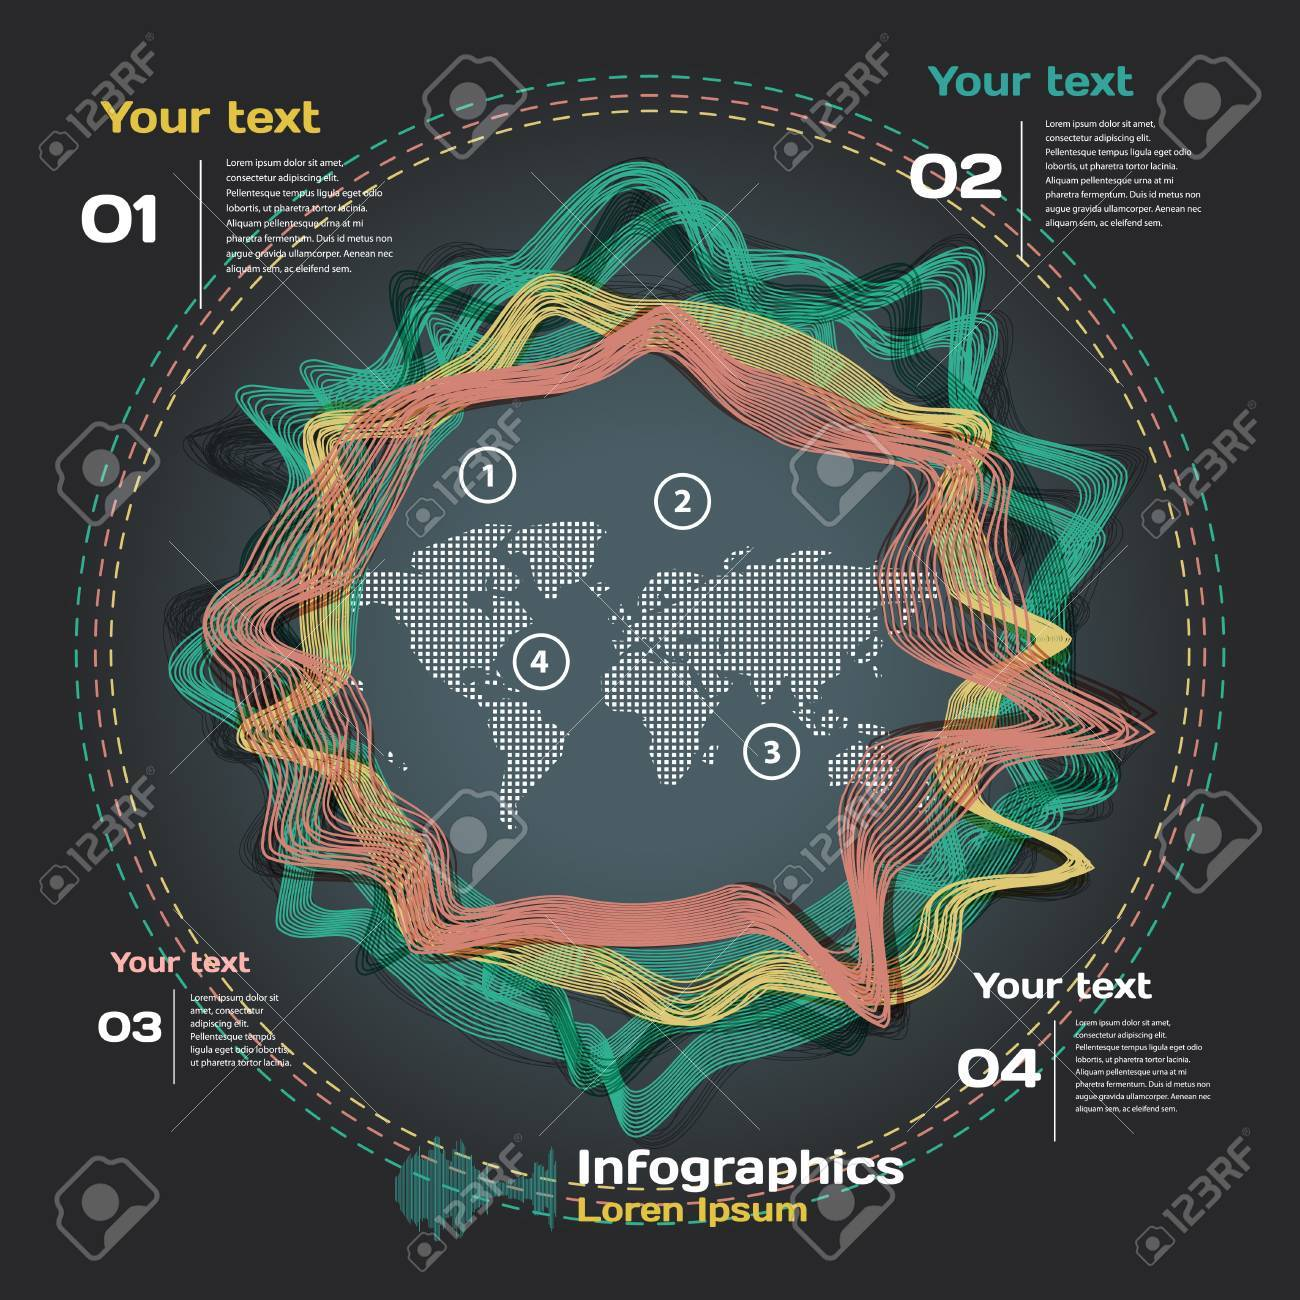
\includegraphics[width=0.33\textwidth]{doc/img/circular.jpg}} 
    \subfigure[]{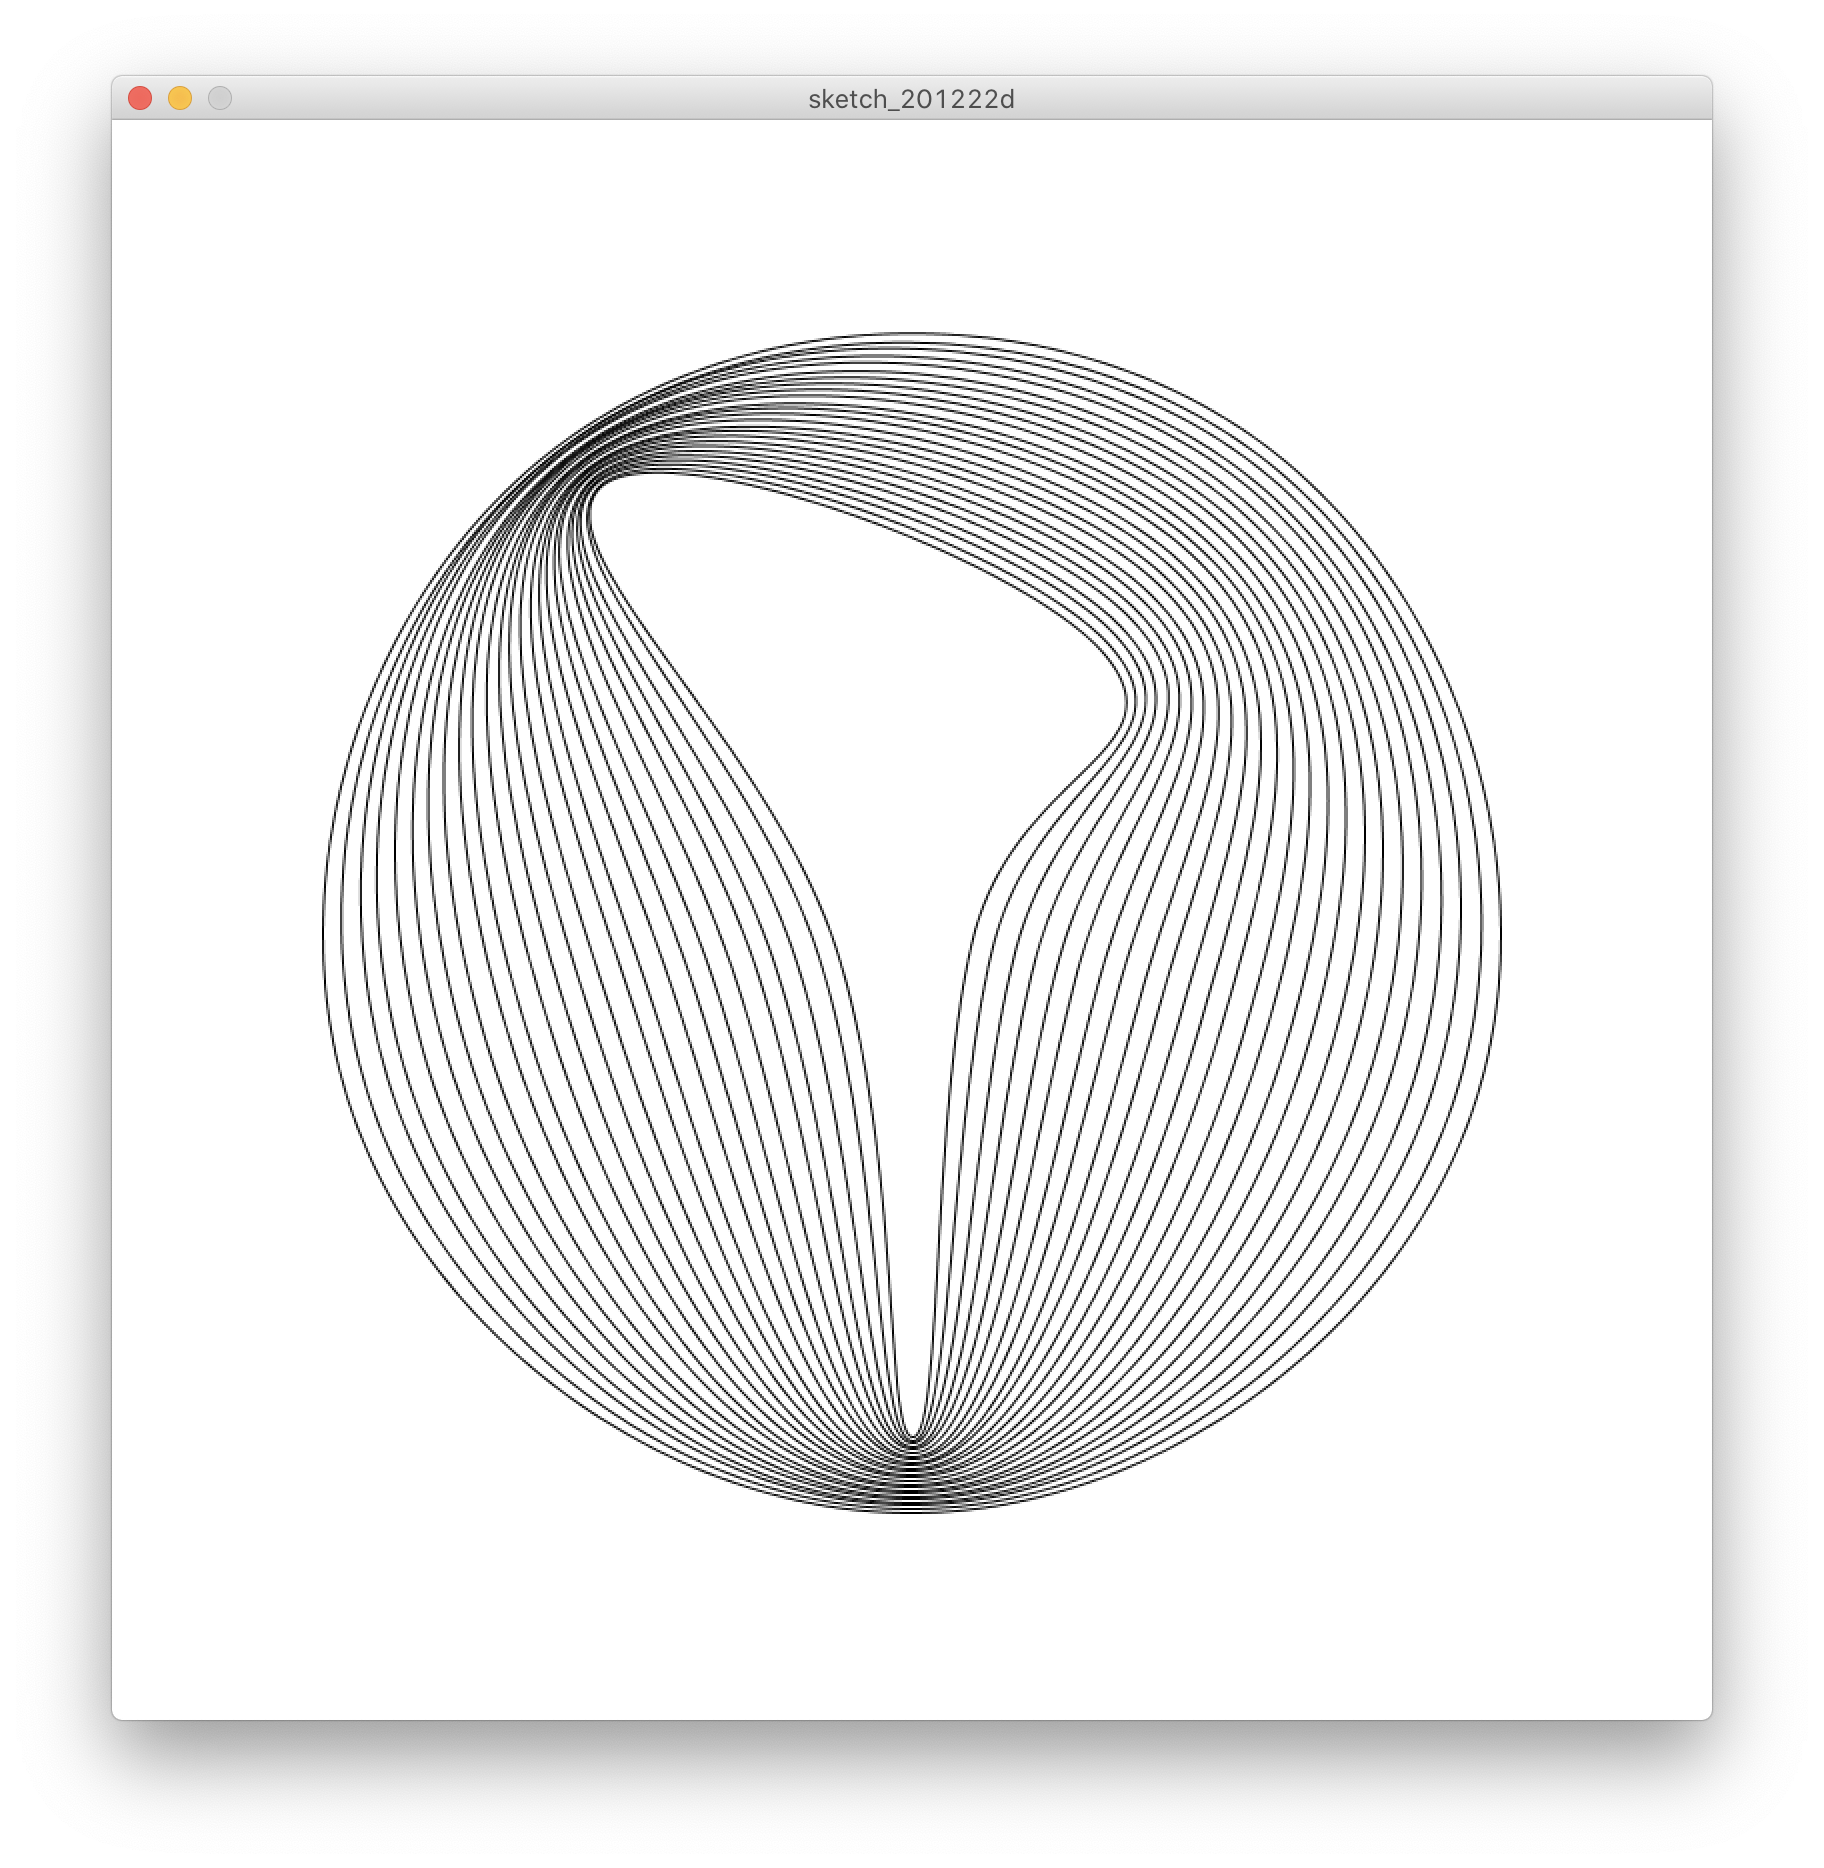
\includegraphics[width=0.33\textwidth]{doc/img/density-plot.png}} 
    \caption{(a) Word frequency per Document \href{https://www.123rf.com/photo_36990141_stock-vector-infographics-with-sound-waves-on-world.html}{Copyright to Vladimir Arkatov} (b) \label{density-plot} Our Implementation}
    \label{fig:circle-digram}
\end{figure}

xxxxxxx
Calculating the position of points in a circle
\href{https://stackoverflow.com/questions/5300938/calculating-the-position-of-points-in-a-circle}{Stackoverflow}


curveVertex
dabei werden die Punktkorrdinaten auf einem Kreis berechnet und danach einzeln mittels vertex kurve verbunden



\begin{figure}
    \centering
    \subfigure[]{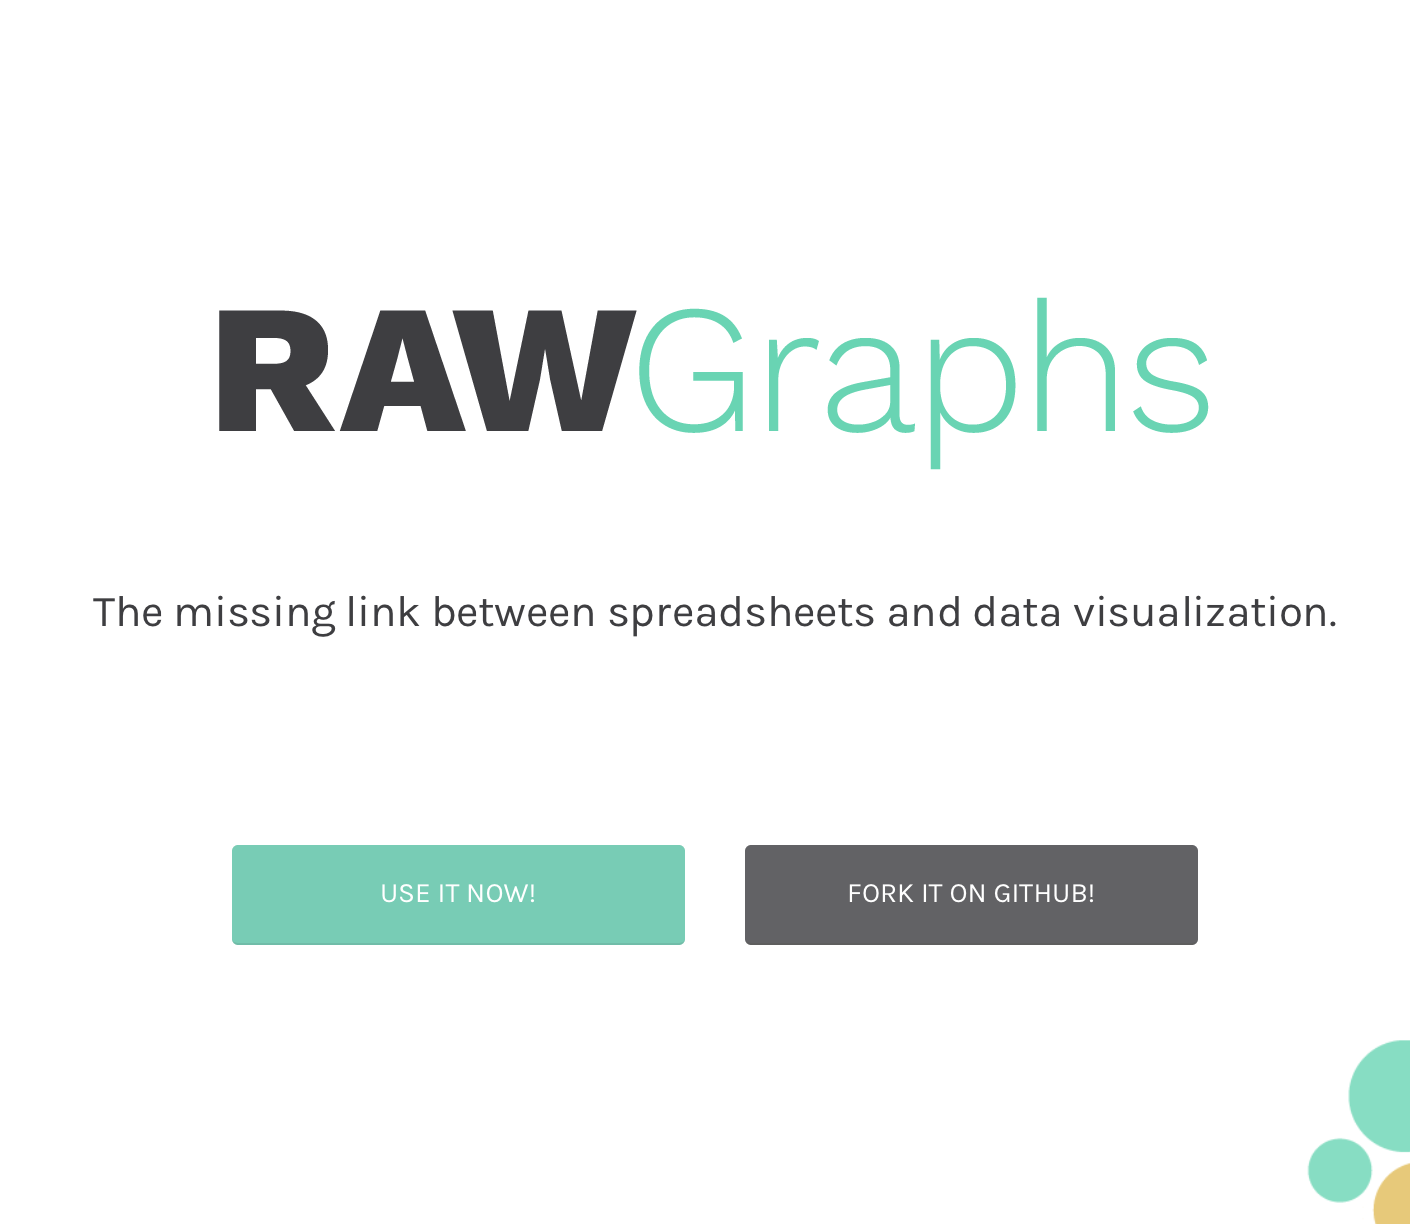
\includegraphics[width=0.33\textwidth]{doc/img/raw.png}}
    \subfigure[]{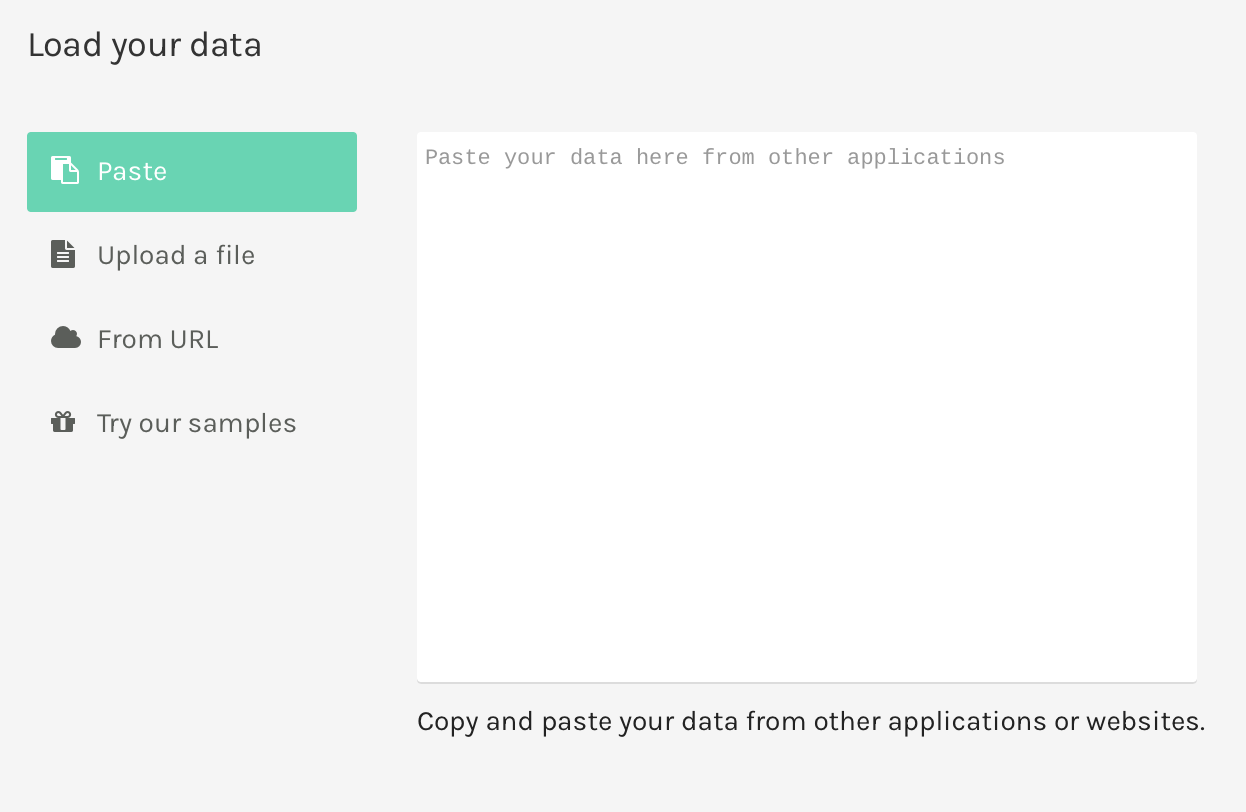
\includegraphics[width=0.33\textwidth]{doc/img/raw-02.png}}
    \caption{\href{https://rawgraphs.io}{Userinterface from RawGraphs-processing}}
    \label{fig:website-reference}
\end{figure}


%>>>>>>>>>>>
%------------------------------------------------------------------------------------- (Implementation)
\section{Implementation}
Based on research process, we started to build up our fingerprint-implementation which should provide the user a clean look and feel (of the interface), while being also able to easily handle interactive data exploration.

\begin{figure}
    \centering
    \subfigure[]{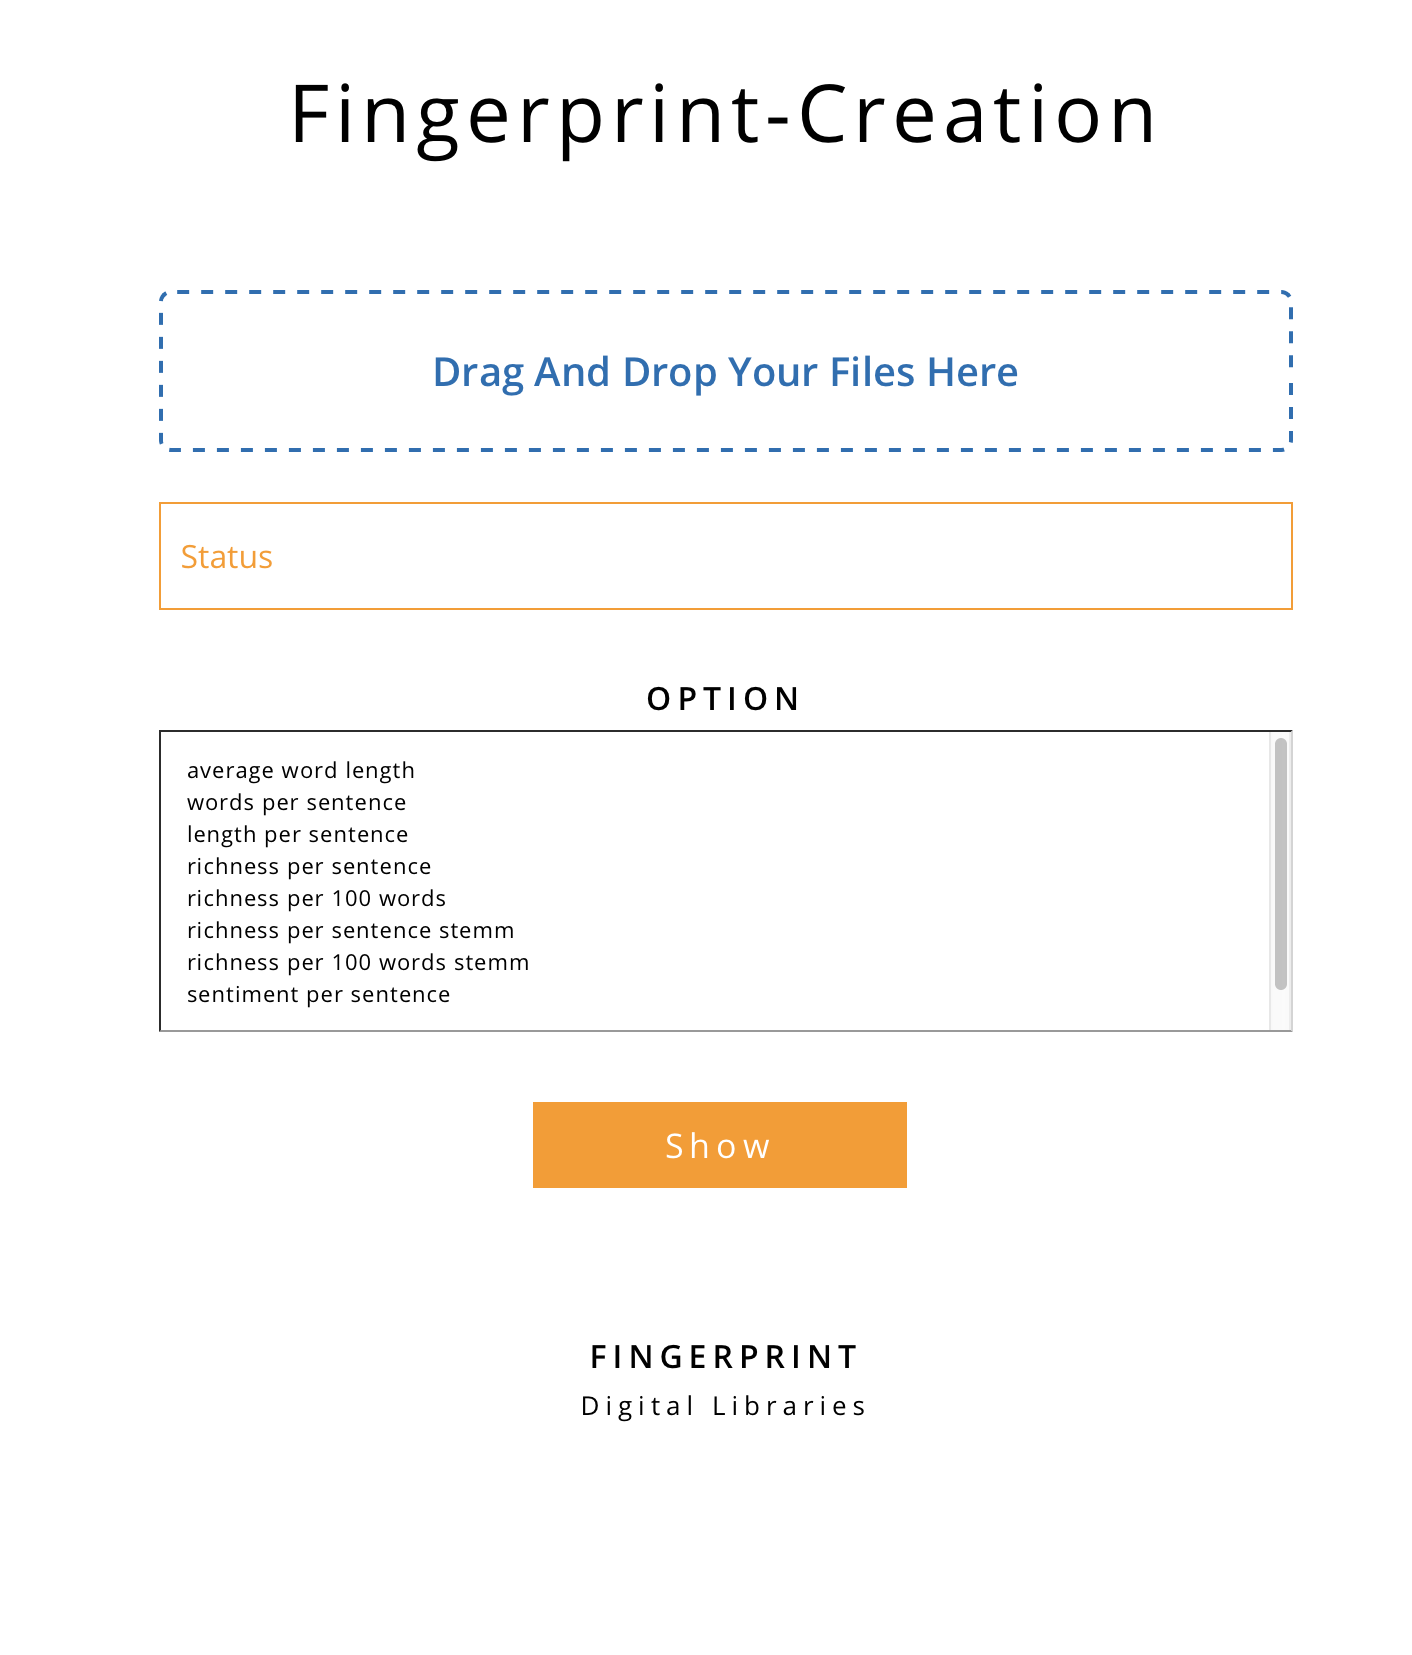
\includegraphics[width=0.33\textwidth]{doc/img/startpage.png}}
    \subfigure[]{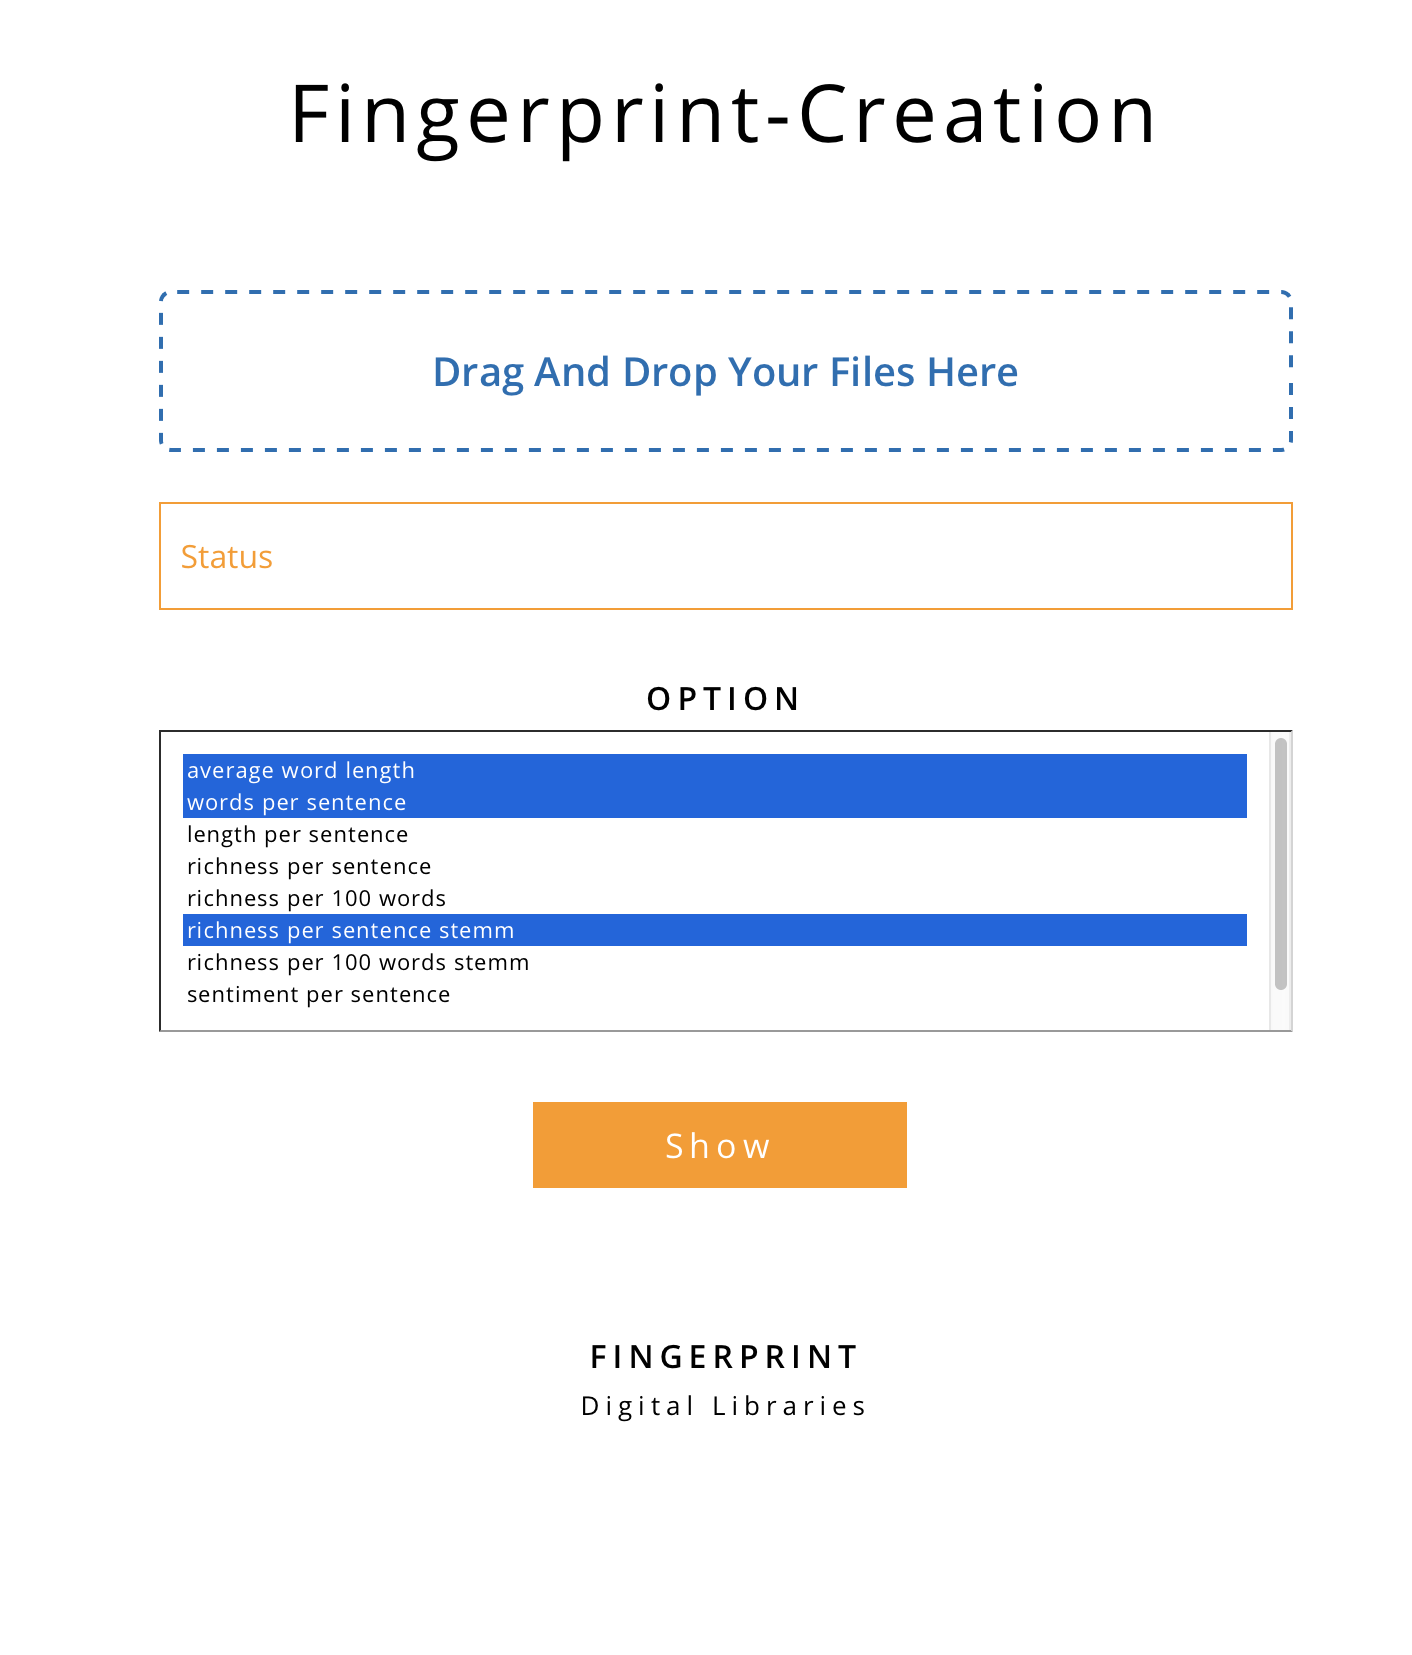
\includegraphics[width=0.33\textwidth]{doc/img/multi-selection.png}}
    \caption{(a) Startpage (b) multi feature selection}
    \label{fig:gui}
\end{figure}

%------------------------------------------------------------------------------------- (DEV-Environment)
\subsection{Development environment (language, libraries, ...)}

\begin{itemize}
    \item \href{https://www.python.org/downloads/}{Python3}
    \item Python3 libraries
    \begin{itemize}
        \item socketserver
        \item http
        \item time
        \item os
        \item platform
        \item numpy
        \item nltk
        \item sys
        \item platform
        \item glob
        \item seaborn
        \item matplotlib
        \item pandas
    \end{itemize}
    \item Visual libraries 
    \begin{itemize}
        \item D3
        \item P5 (legacy) it was used for circular density-plot (see Fig. \ref{density-plot})
    \end{itemize}
    \item Web Browser
    \begin{itemize}
        \item \href{https://www.mozilla.org/de/firefox/new/}{Firefox 84.0.2}
    \end{itemize}
    \item IDE
    \begin{itemize}
        \item \href{https://www.jetbrains.com/de-de/pycharm/}{pyCharm}
    \end{itemize}
\end{itemize}


%------------------------------------------------------------------------------------- (Implemented Functionality)
\subsection{Implemented functionalities/features}

\begin{itemize}
    \item Feature extraction
    \begin{itemize}
        \item words per sentence
        \item length per sentence
        \item richness per sentence
        \item richness per 100 words
        \item richness per sentence stemm
        \item richness per 100 words stemm
        \item sentiment per sentence
        \item digit count per sentence
    \end{itemize}
    \item Drag \& Drop
    \begin{itemize}
        \item single Feature selection
        \item multi Feature selection
    \end{itemize}
    \item dynamic and interactive visual representation of calculated data in a 20 to 20 matrix 
    \begin{figure}
        \centering
        \subfigure[]{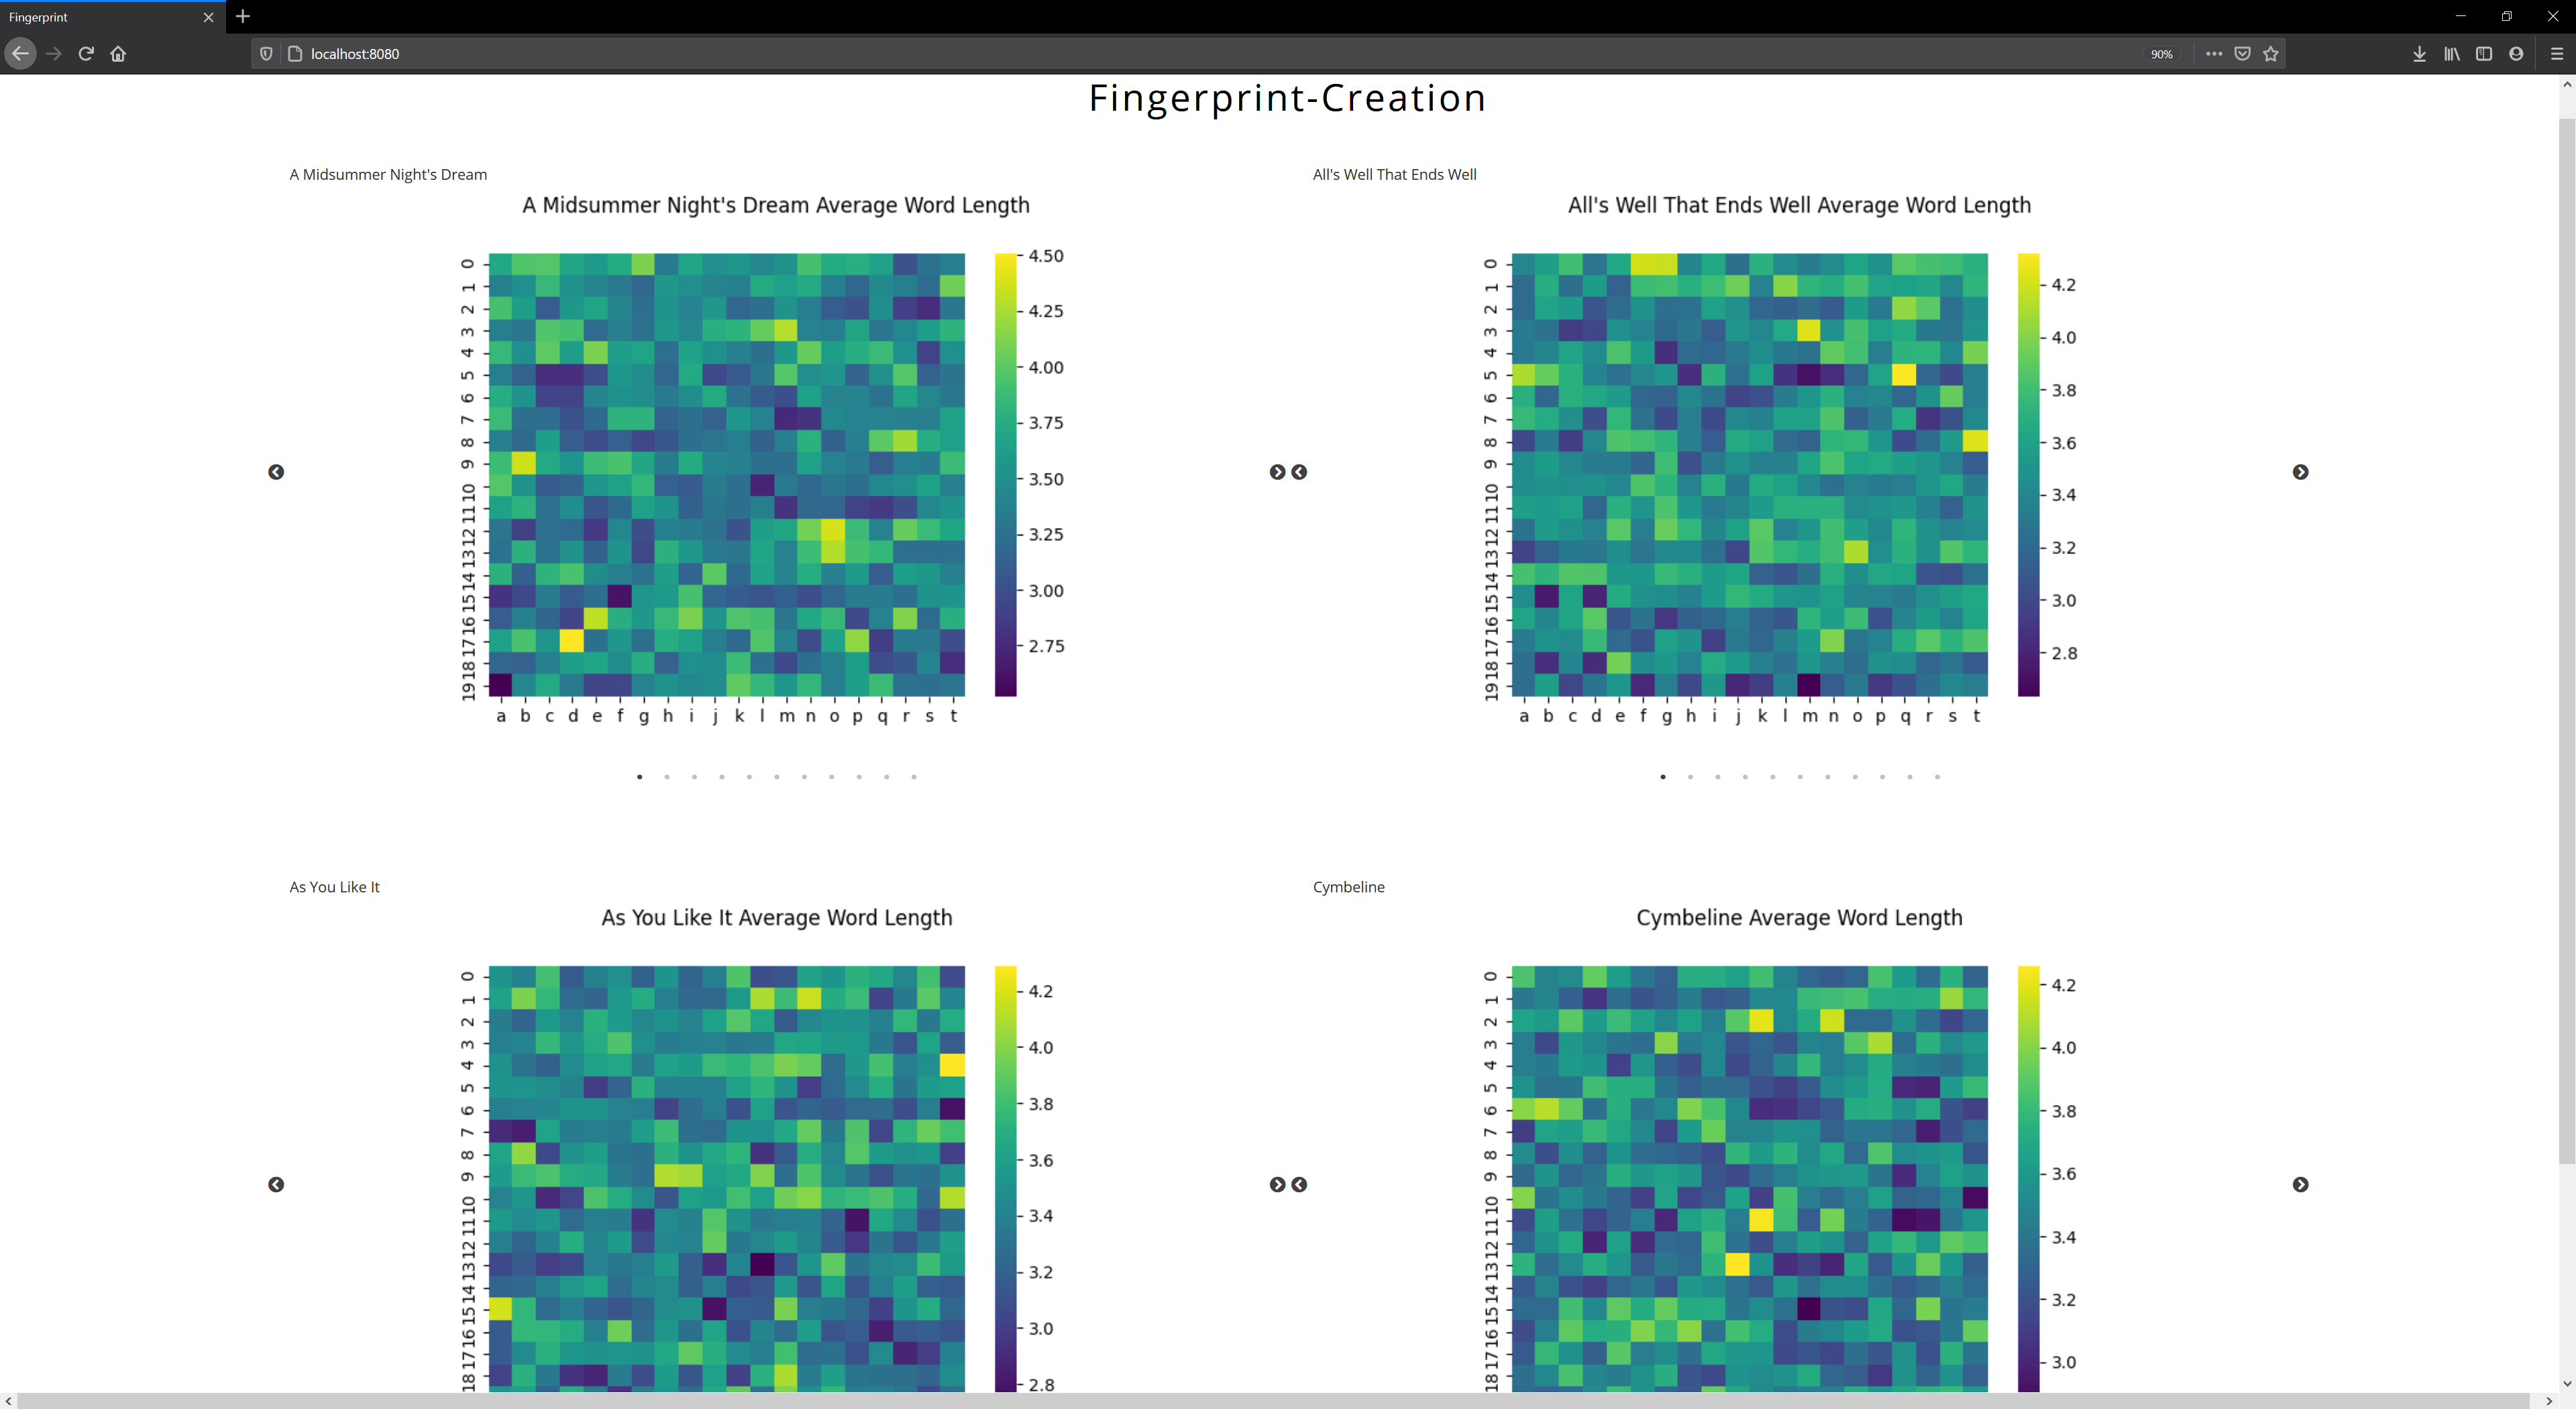
\includegraphics[width=0.51\textwidth]{doc/img/result/server-result.png}} 
        \caption{(a) mutiple results for multiple files}
        \label{fig:heatmap}
    \end{figure}
    \item metadata information by driving over a field. \\
    \textbf{Note} At the moment deactivated. The reason was a strange beahaviour from D3 which only did that for one file, when multiple files where calculated.
    \begin{figure}
        \centering
        \subfigure[]{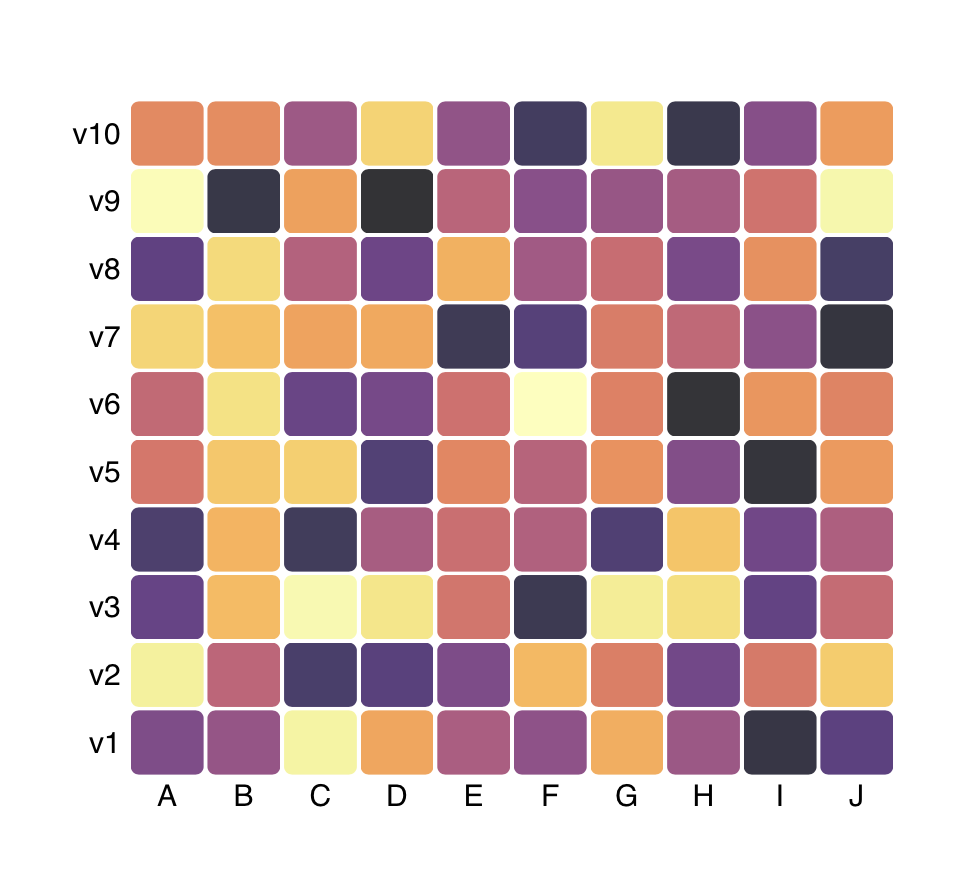
\includegraphics[width=0.24\textwidth]{doc/img/heatmap-without-meta.png}} 
        \subfigure[]{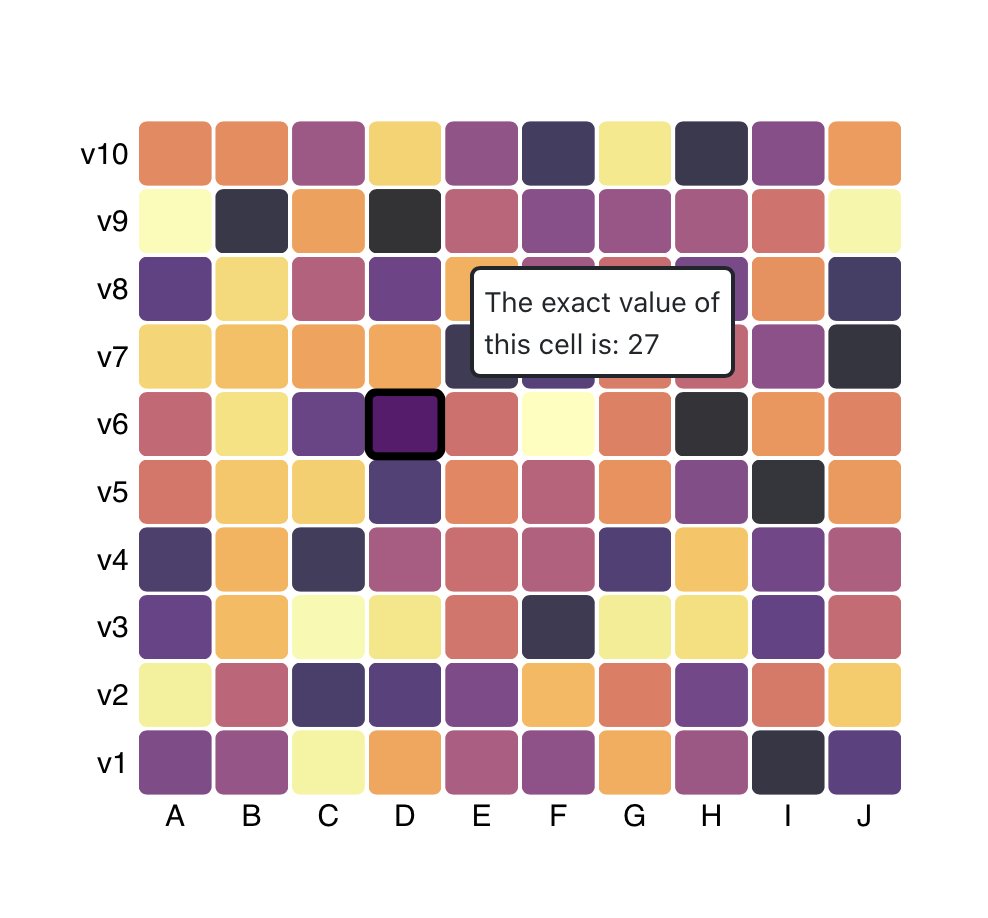
\includegraphics[width=0.24\textwidth]{doc/img/heatmap-with-meta.png}}
        \caption{(a) Heatmap without metadata (b) Heatmap with metadata}
        \label{fig:metdata}
    \end{figure}
\end{itemize}



%------------------------------------------------------------------------------------- (Implemented-Userflow)
\subsection{Description of supported user operations (workflows)}
Front-End:
\begin{itemize}
    \item file drag \& drop to the system
    \item single-feature-selection
    \item multi-feature-selection
    \item interactive GUI
    \item responsive GUI
\end{itemize}
Back-End:
\begin{itemize}
    \item Feature Extraction \\
    Using NLP, we should be able to obtain features from a given text. Features such as word length, sentence length, sentiment of a sentence, etc\ldots We developed the file \texttt{feature\_extraction.py} to take care of just that. We used the programming language \texttt{Python} for this task due to it being incredibly powerful and easy to use in data-related tasks. Furthermore the \texttt{Natural Language Toolkit} library is supported by \texttt{Python}. This tool allows the programmer to use symbolic and statistical natural language processing for the English language.
    \item Natural Language Toolkit \\
    The \texttt{Natural Language Toolkit} (or NLTK) library is downloaded and installed into one's \texttt{Python} environment through the following line of code:
    %------------------------------------------------------------------------------------- (Python-NLTK-1)
    \lstinputlisting[language=Python]{doc/src/nltk-1.py}
    From the NLTK library we use the following functions:
    \begin{itemize}
        \item Sentence Tokenizer: from a text, return a list of the entire text separated per sentence.
        \item Word Tokenizer: from a text, return a list of the entire text separated per word.
        \item Porter Stemmer: from a given word, return the root of it using a Porter Stemmer algorithm.
        \item Stop Words: returns a list of all stop words from the English language (words with no inherent meaning - such as the words "the" and "a".)
        \item Sentiment Intensity Analyser: from a sentence, return a dictionary containing the negative, neutral, positive, and compound values from that sentence.
    \end{itemize}
    We imported them into our \texttt{Python} file as such:
    %------------------------------------------------------------------------------------- (Python-NLTK-2)
    \lstinputlisting[language=Python]{doc/src/nltk-2.py}
\end{itemize}
We will now elaborate on two method functions of the supported. One of them is able to extract features from the document, and the other is able to package the results into a format useful for heatmap creation.
%------------------------------------------------------------------------------------- (Python-getAverageWordLengthPerXWords)
%\lstinputlisting[language=Python]{doc/src/getAverageWordLengthPerXWords.py}

In the function \texttt{getAverageWordLengthPerXWords}, we are trying to get the average word length every \texttt{x} amount of words. To do this, we must first tokenize the \texttt{parameter} using a tokenizer from the NLTK library. The variables \texttt{tokens} contains a list of all words in the text. We then iterate through the words. At every word, we increase our word counter variable \texttt{word\_count} by one and our word length counter \texttt{word\_len} by the size of the current word we are looking at. Notices that we are only looking at words that are not exclusively a punctuation. Once our \texttt{word\_count} counter reaches \texttt{x}, then we append the value of the \texttt{word\_len} variable divided by our \texttt{x} onto our \textit{result} list. We then reset our two counter variables. Once we have gone through all words, if there are words that we have not accounted for yet, we append them now. Finally, we return our \texttt{result} list. This list will contain the average length of words every \texttt{x} words. 

The other features follow a similar structure. If we want to get the average sentence length per \texttt{x} words, we would follow the snippet above but change the tokenizer method from using the word tokenizer to the sentence tokenizer. If we cared about getting the average sentence length of every length, we disregard the counters and the \texttt{x} variable. If we wanted to calculate richness, we would stem the words using the Porter Stemmer, which computes the ``roots" of words. We then count unique words. To calculate sentiment, we tokenize sentences and then pass them through the sentiment analyzer from the NLTK library. This returns a dictionary with values for positive, negative, neutral, and compound sentiment.

The next step in our feature extraction script is to grab this resulting list and converting it into an $\texttt{n} \times \texttt{n}$ matrix. In our demo, we set our \texttt{n} to $20$. The way we did it can be seen in the snippet below.

%------------------------------------------------------------------------------------- (Python-chunkList)
%\lstinputlisting[language=Python]{doc/src/chunkList.py}


The function \textbf{chunkList} grabs a value for \texttt{n} and an array. We want to turn this list into a list of \texttt{n} lists each consisting of \texttt{n} amount of elements. To do this, it first compute the \texttt{avg} variable. This variable lets the algorithm how many elements of the array should be grouped together to end up with our required size. It divides the length of the array by $\texttt{n}^2$. The \texttt{while} loop iterates through the array initially grouping an \texttt{avg} amount of elements, grabbing the mean and appending it onto a \texttt{tmp} list. The \texttt{last} variable is added with \texttt{avg}. In the next iteration, the loop groups an \texttt{avg} amount of elements starting from the \textit{last} index. This is done \texttt{n} times. Once this occurs, the \texttt{tmp} list, which now contains \texttt{n} elements is added to the \texttt{result} variable. The \texttt{tmp} list is then reset. The loop continues until the \texttt{result} variable is of size $\texttt{n} \times \texttt{n}$ and the list is returned. 

This $\texttt{n} \times \texttt{n}$ list is fed to another script which is focused on creating a heatmap based off of the values in this list. For the chunking of the sentiment of words, since we get a dictionary, we grab the first values of all dictionaries and put them into one list, then another list for the second value in the dictionary, and same for the third list and value. We then chunk all three lists as we do the other lists. 


%------------------------------------------------------------------------------------- (Demo)
\section{Application demonstration}


%------------------------------------------------------------------------------------- (Demo-walkthrew)
\subsection{Demonstrate the supported user operations by a walkthrough of a hypothetical user Alice considering the used data}
\begin{figure}
    \centering
    \subfigure[]{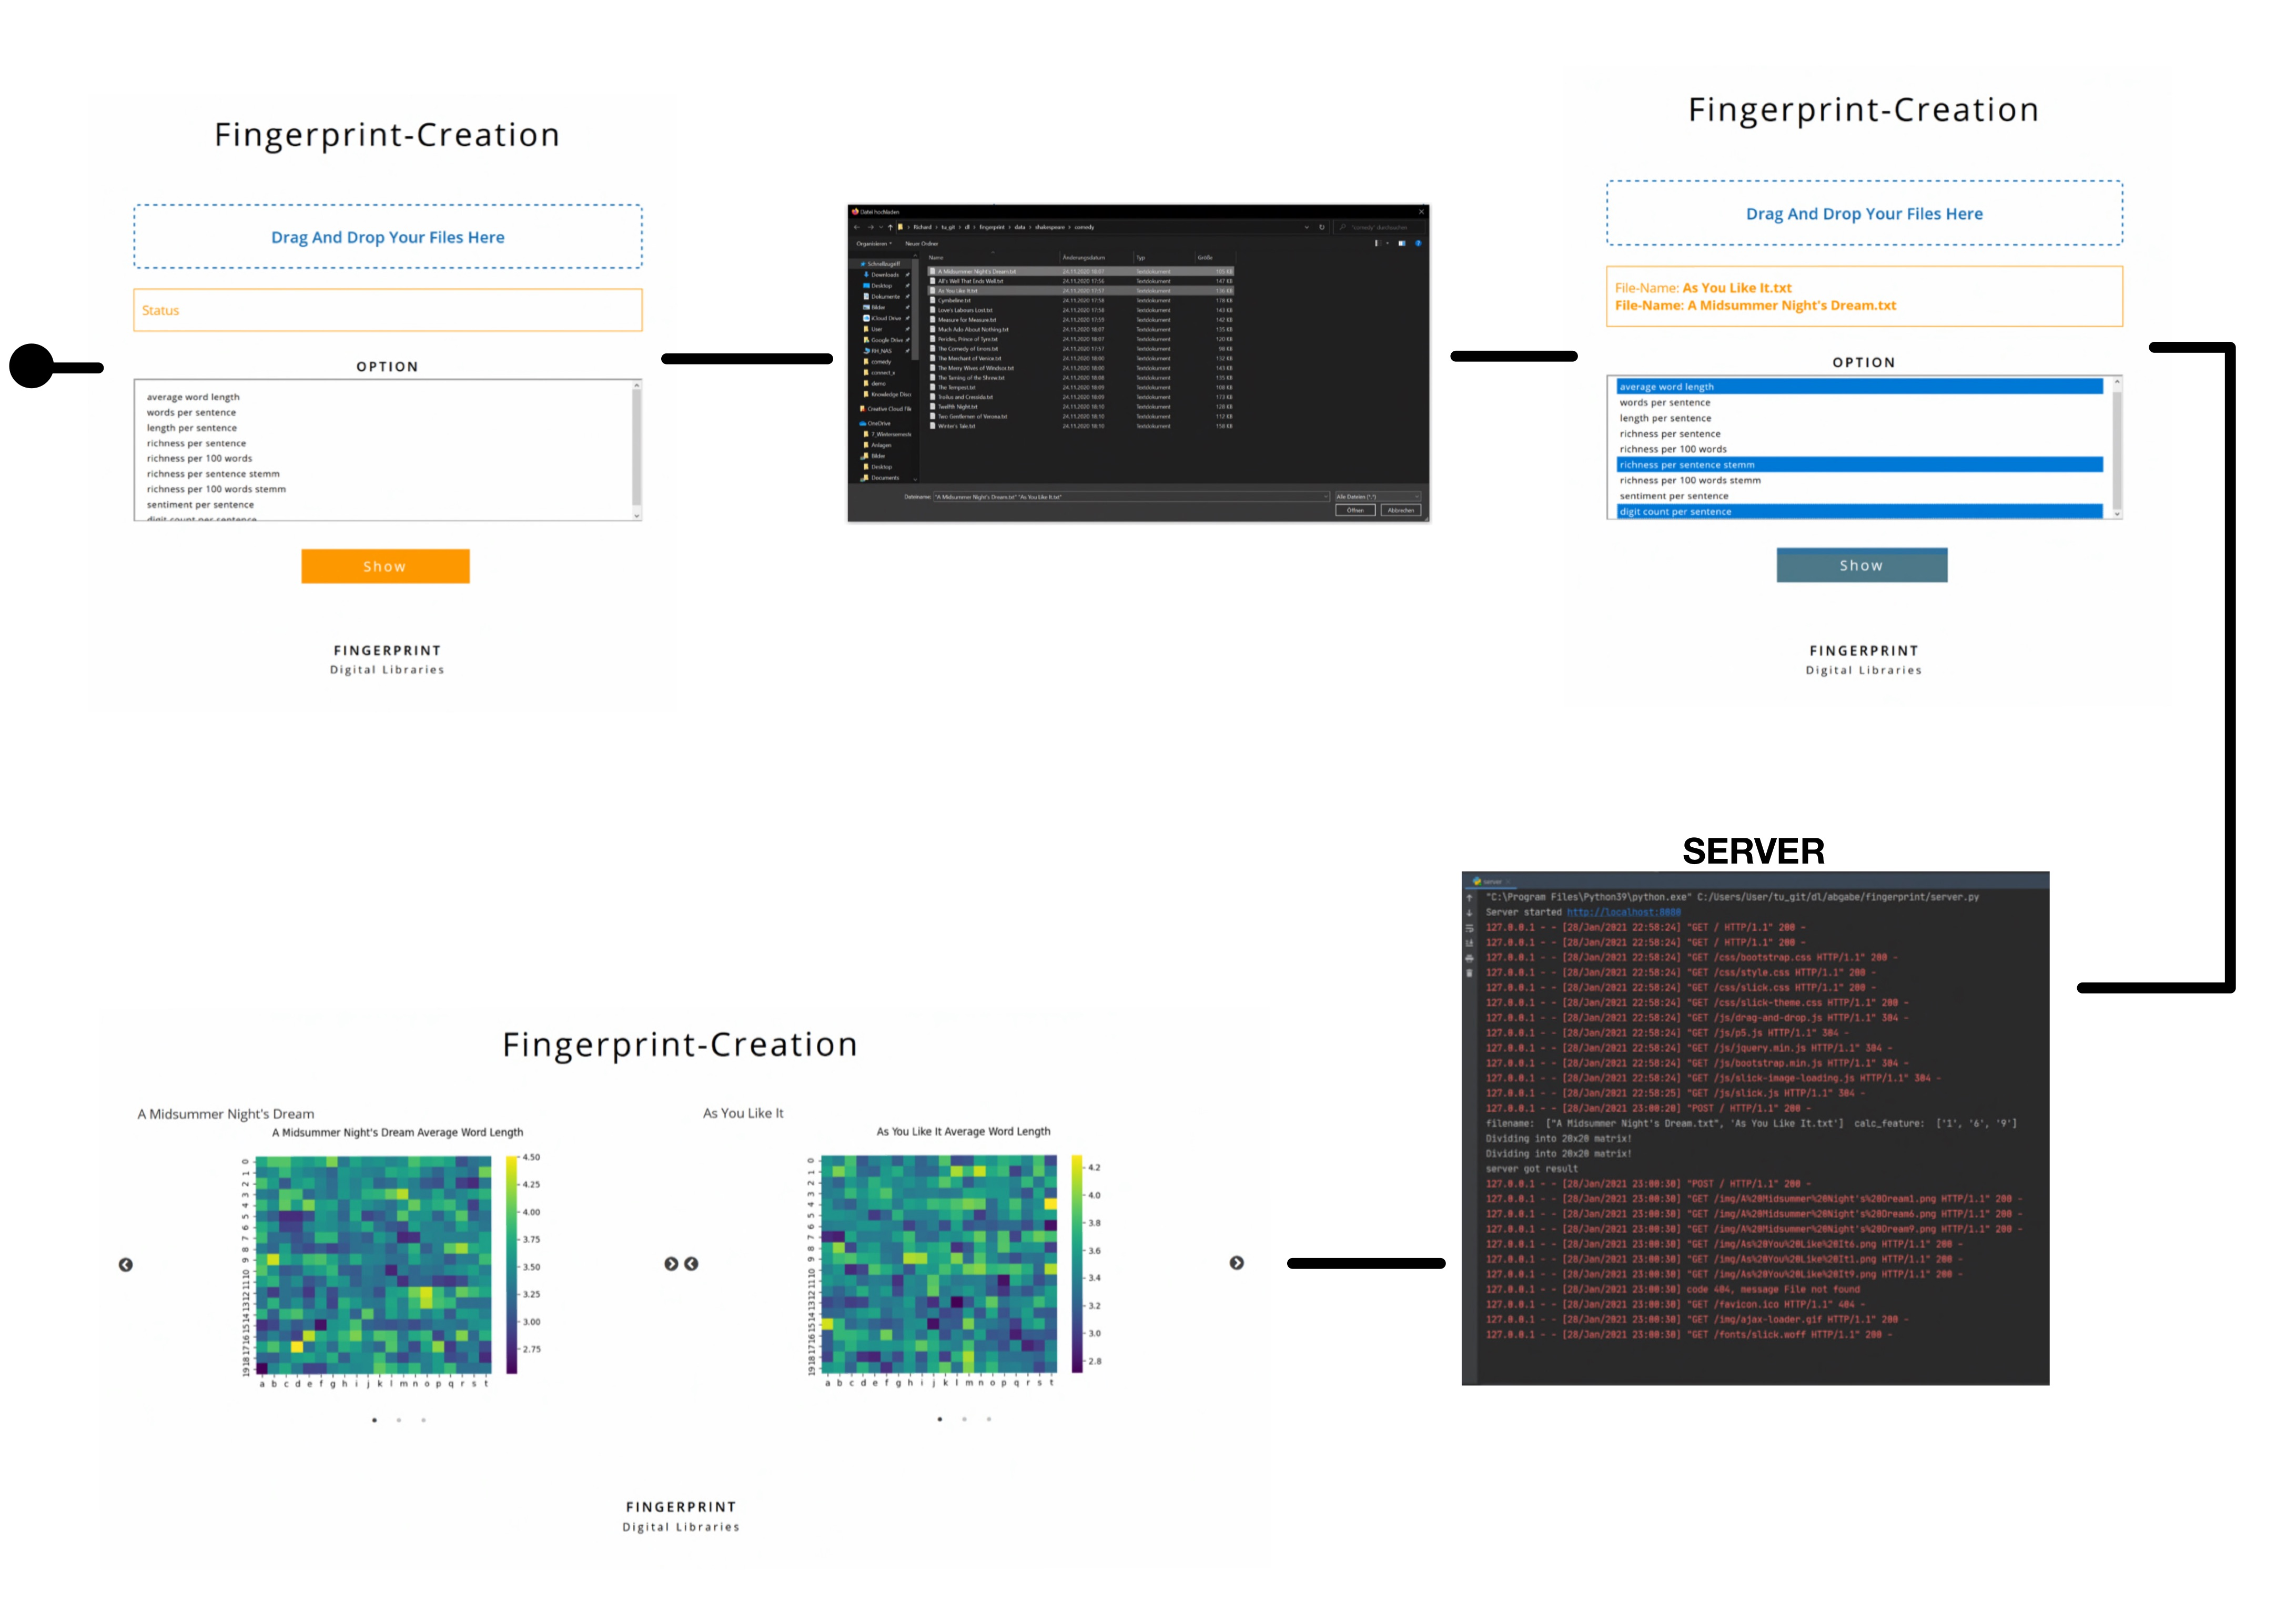
\includegraphics[width=1\textwidth]{doc/img/process.jpg}} 
    \caption{(a) The overall user process and calculatin flow}
    \label{fig:overall process}
\end{figure}
The overall process is, that the user starts the server 


%------------------------------------------------------------------------------------- (Demo-Exploration)
\subsection{Describe how and where searching and exploring are possible}

When the pipeline is run through the calculated heatmap-results are shown up in a grid layout. Giving the user the ability to visually analyse and compare them just side by side. Even the comparison of multiple features for one file is possible, if the user loads the file more than once.
\begin{figure}
    \centering
    \subfigure[]{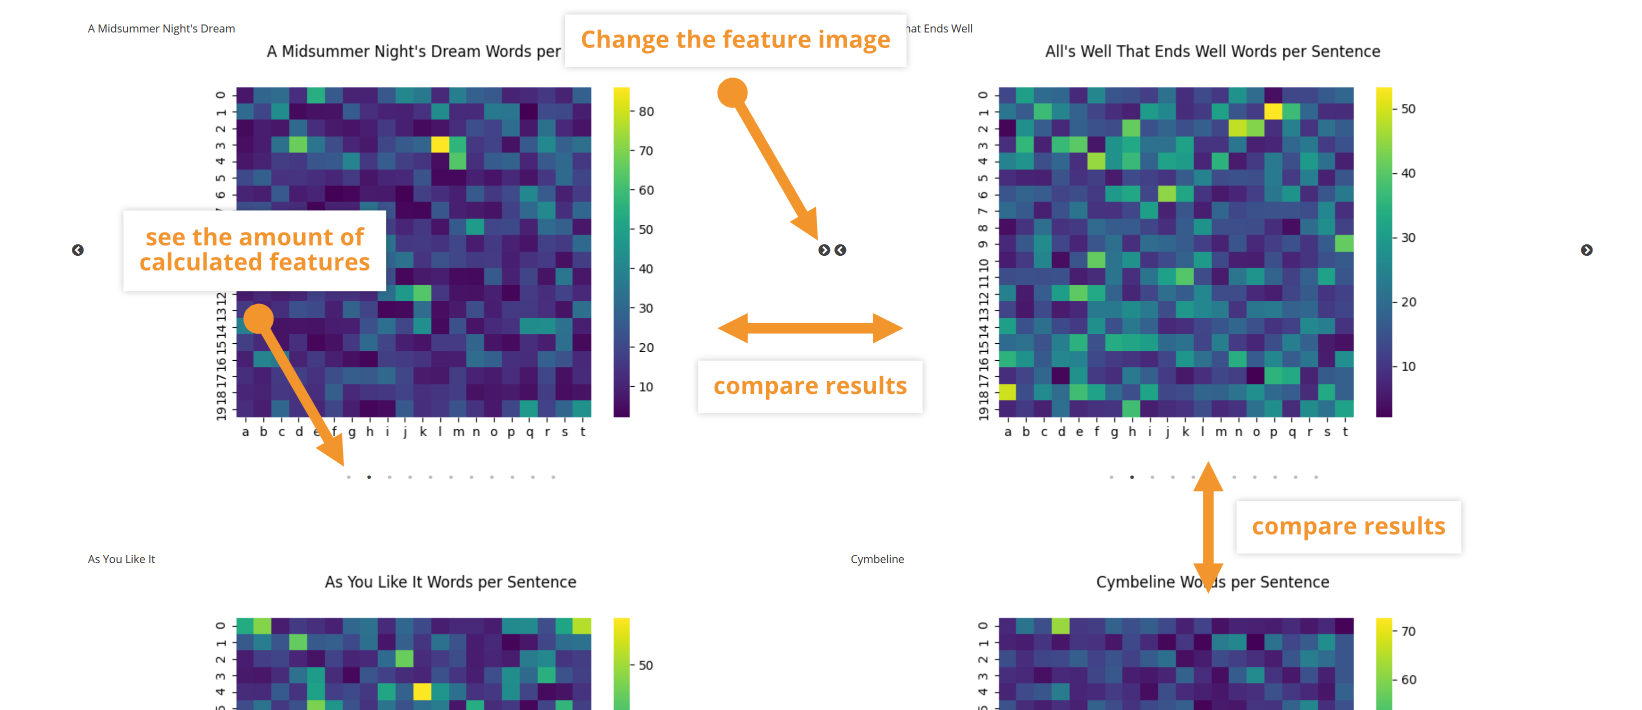
\includegraphics[width=1\textwidth]{doc/img/result/analysis-explaination.png}} 
    \caption{(a) Analysis overview}
    \label{fig:process analysis}
\end{figure}

XXXXXXXXX
gab es data preparation, wir haben die daten ausgegeglidert.


%------------------------------------------------------------------------------------- (Demo-Findings)
\subsection{Describe interesting findings and observations you made when applying your solution to the data}
As you can see, the comparison of two comedy works shows a significant difference between the sentence length.

\begin{figure}
    \centering
    \subfigure[]{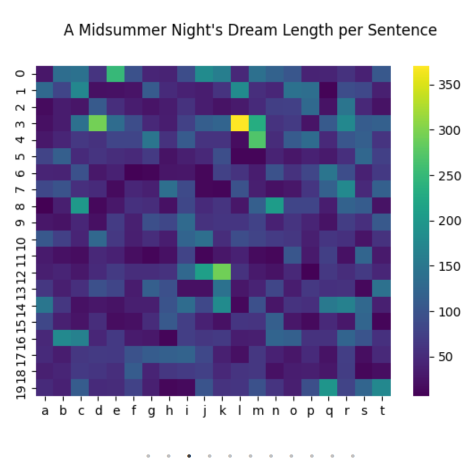
\includegraphics[width=0.4\textwidth]{doc/img/result/compare1.png}}
    \subfigure[]{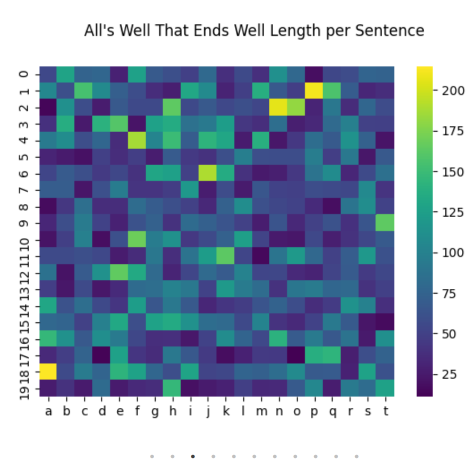
\includegraphics[width=0.4\textwidth]{doc/img/result/compare2.png}}
    \caption{(a) Comedy (b) Comedy}
    \label{fig:foobar}
\end{figure}

Also a significant difference was visible by comparing:
\begin{itemize}
    \item history against poetry
    \item comedy-charakter-1 against comedy-charakter-2 \\ meaning that one used long-and the otherone short-words.
    \item history used more numbers and dates compared to other documents
    \item different characters \\ meaning that some talk more than others.
\end{itemize}


%>>>>>>>>>>> Hauptpunkt
%------------------------------------------------------------------------------------- (advantages, limitations and future)
\section{Discussion of advantages, limitations and future developments to do}
The whole system enables the user to:
\begin{itemize}
    \item[+] easily detect significant outliers
    \item[+] process more than one files at once
    \item[+] calculate more than one feature
    \item[+] compare different file at once
    \item[+] use it also as web-app (mobile)
    \item[+] use a clean designed GUI
    \item[+] save heatmap results as image
    \item[+] be platform independent because of client server architecture
    \item[+] there is no file amount limitation \\ \textbf{hint}: the more files the longer calculation takes
    \item[+] take a look at the entire work of \href{http://shakespeare.mit.edu/}{William Shakespeare}
    \item[--] process only TXT-files
    \item[--] use Firefox on desktop
    \item[--] only see static images \\ interactive version is deactivated in background
    \item[--] not see the direct reference to the text
    \item[f] reference from heatmap to text
    \item[f] even better interactivity with the results \\e.g. sorting, drag\&drop of results
    \item[f] see metadata
    \item[f] Handle the Browser-cache-Flash after sending it to the server
    \item[f] automatically detect the text-genre \\e.g. historic or  non-historic text
\end{itemize}

+ \ldots Advantage / -- \ldots Limitation / f \ldots Future


%------------------------------------------------------------------------------------- (Contribution)
\section{Contributions}
\begin{itemize}
  \item Richard Hohensinner \\ (design, coding, application, report writing)
  \item Inti Gabriel Mendoza Estrada \\ (design, coding, application, report writing)
  \item Jürgen Suntinger-Schrampf \\ (design, coding, application, report writing)
\end{itemize}


%------------------------------------------------------------------------------------- (References)
%% BibTeX users should specify bibliography style 'splncs04'.
%% References will then be sorted and formatted in the correct style.
%%
\bibliographystyle{splncs04}
\bibliography{bookReferences.bib}


%
%da eine onlineplatofrm für fingerprints naschauen, einen host
%https://www.semanticscholar.org/paper/Literature-Fingerprinting%3A-A-New-Method-for-Visual-Keim-Oelke/474178dae941d135190ba98cfb7c3aa67924b09b
%https://www.dw.com/en/whodunit-how-fingerprinting-has-inspired-writers/a-19516521
%https://physicsworld.com/a/literary-fingerprints/
%The foundation of our design was the result of three references






\end{document}

